%Introduction Pragraph
The dummy kit has been purchased and built. Our main factor, for the kit, is the fact that it behaves like a vehicle but interacts with the environment. The way it does that is with a multi-directional (Horizontally) sonar (attached to servos) to replicate the front part of our project.\par

\begin{comment}
\subsection{Material List}
We have drafted a complete material list and are ready for unexpected errors/malfunctions that we may face during the design phase. The project's has taken a turn for the better by decreasing the its size by 1 ft of difference compared to our abstract build. We've removed the concept of using dual blades and applied a singular mower blade for less voltage usage and size decremental, making our project possible without having a crazy powerful battery. We've decided that our project won't have a GPS/RTK Base station, due to the fact that we can simply implement the module to the robot itself, and a 2D LIDAR due to our design choices, leading to less expenses.\par
\begin{table}[H]
   \begin{tabular}{|c|c|} \hline 
   \centering
    \textbf{Item}& \textbf{Quantity}\\ \hline
       ESP32-WROOM-32& 1\\ \hline   
       L298N Motor Driver& 1\\ \hline
        Gear Motor 300 RPM 12V& 3\\ \hline 
       Voltage Regular (XL6009)&1\\ \hline 
        Jumper Wires (120 pc)&1\\ \hline 
        20 Gauge Hookup Wires&1\\ \hline 
        Fuse Holder&1\\ \hline 
        Drive Wheel&1\\ \hline 
        Caster Wheel&1\\ \hline 
        10" Cooling Fan&1\\ \hline 
        Ultrasonic Distance Sensor&8\\ \hline 
        GPS/RTK Module&1\\ \hline 
        Rain Sensor Module&1\\ \hline 
        Power Switch&1\\ \hline 
        Battery&1\\ \hline
        Wire Holder&2\\\hline
        Pixhawk PX4 Flight Controller&1\\\hline
    \end{tabular}
    \caption{Material List as of \today} 
    We can do either \today if we want to have it constantly updating or we can just make it October 21, 2024
\label{tab:table1}
    
\end{table}
\end{comment}

 
\subsection{Design}
The project's outer design was talked through during our first meeting. Agreeing that its outer shell will take the shape of a cylindrical ring, where the blade and fan are placed at the middle part. This design idea was to excel the vacuum performance of the fan, pulling the grounded grass to then push the cut ones simultaneously. That being said, we sacrificed the LIDAR to embrace its unique design, using a total of 6-8 sonar sensors to try and replicate the LIDAR's dynamic approach. In addition, the design must also be created with a UV resistant material. ASA (Acrylonitrile Butadiene Styrene) is our current pick for this use, as it is a UV resistant material, and is easily outsourced to fit our needs for 3D printing. Autodesk Fusion 360 is currently being used to model this outer shell prototype.\par

\begin{figure}[H]
    \centering
    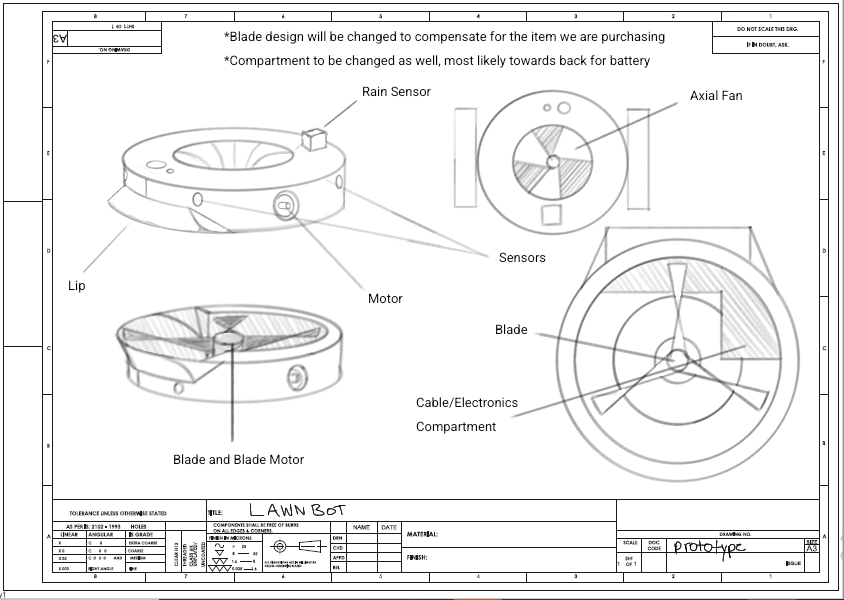
\includegraphics[width = 0.8\textwidth]{root/Lawn_Bot_V1.jpg}
    %\includegraphics[width = 0.2\textwidth]{root/UB-Seal.eps}
    \caption{LawnBot Design (\today)} 
    \label{fig:LawnBot_Design_V1}
\end{figure}


\subsection{Testing Phase}
Realizing the material list's delivery date, we purchased a kit to test on, containing a similar microcontroller, to start the software and wiring testing/implementation. This will speed up the process into understanding the automation field of the project and start the testing phase of our project while helping us plan ahead once we get our actual equipment. \par